\section{空间的构造}
\label{sec:topo-constructions}

很多空间是从已有空间造出来的：圆周是平面的一部分，随时间运动的位置取值于“空间乘以时间”，圆周也可以由线段把两端粘合得到。这三种构造各有一个自然的映射，即包含映射、坐标投影和商映射。新空间的开集，就按“使这个映射连续”来规定，这条规则同时给出了判断映入或映出新空间的映射何时连续的方法。

\subsection{子空间}
\label{sec:topo-subspaces}

研究圆周$S^1=\{(x_1,x_2)\in\mathbb R^2:x_1^2+x_2^2=1\}$时，我们希望沿用平面的“附近”：圆周上一点附近，就是平面上这点附近与圆周的公共部分。

\begin{definition}[子空间拓扑]
\label{def:topo-subspace}
设$(X,\mathcal T)$是拓扑空间，$A\subseteq X$。下面的族是$A$上的拓扑，称为\term{子空间拓扑}（subspace topology）：
\begin{equation}
 \mathcal T_A=\{U\cap A:U\in\mathcal T\}.
 \label{eq:topo-subspace}
\end{equation}
称$(A,\mathcal T_A)$为$X$的子空间，$\mathcal T_A$的成员称为在$A$中\term{相对开}（relatively open）的集合。
\end{definition}

$\mathcal T_A$确实是拓扑：$\varnothing\cap A$与$X\cap A$分别给出$\varnothing$与$A$，并且
\[
 \bigcup_i(U_i\cap A)=\Bigl(\bigcup_iU_i\Bigr)\cap A,\qquad
 (U\cap A)\cap(V\cap A)=(U\cap V)\cap A.
\]

对补集取交同样可得：$A$中的相对闭集恰是形如$F\cap A$的集合，$F$为$X$的闭集。若$\mathcal B$是$X$的拓扑基，则$\{B\cap A:B\in\mathcal B\}$是子空间拓扑的基。

\paragraph{相对开与在环境中开}
相对开放比在环境中开放的要求低。取$X=\mathbb R$，$A=[0,1]$。如图~\ref{fig:topo-subspace-wrap}(a)，集合
\[
 [0,1/2)=(-1,1/2)\cap A
\]
在$A$中相对开，在$\mathbb R$中却不开。$A$本身作为子空间是全空间，因而在$A$中既开又闭，在$\mathbb R$中它只是闭集。

端点处的邻域只需单侧：$0$在$A$中的邻域基可以取$[0,1/k)$，$k\geq1$。单点集$\{0\}$在$A$中仍不开，因为每个相对开的含$0$集合都含有某个$[0,\varepsilon)$。

当$A$本身在$X$中开时，相对开集就是含于$A$的$X$的开集，因为两个开集的交仍开。上面的差别只出现在非开的子集上。描述子集的开闭性时，因此必须说明环境：“在$A$中开”与“在$X$中开”是两回事。

\paragraph{映入子空间的映射}
包含映射$\iota:A\to X$，$\iota(a)=a$，是连续的，因为$\iota^{-1}(U)=U\cap A$。子空间拓扑恰好使这一点成立：它是$A$上使$\iota$连续的最粗拓扑。因此，连续映射$f:X\to Y$限制到子空间上仍连续，因为$f|_A=f\circ\iota$。

\begin{lemma}[映入子空间的映射]
\label{lem:topo-map-into-subspace}
设$A\subseteq Y$为子空间，$g:Z\to A$。则$g$连续，当且仅当$\iota\circ g:Z\to Y$连续。
\end{lemma}
\begin{proof}
必要性是复合的连续性。充分性：$A$的每个开集形如$V\cap A$，$V$为$Y$的开集，而
\[
 g^{-1}(V\cap A)=(\iota\circ g)^{-1}(V)
\]
是开集。
\end{proof}

判断一个映入圆周的映射是否连续，只需把它看成映入平面的映射，逐坐标检验。例如$p(t)=(\cos2\pi t,\sin2\pi t)$作为$\mathbb R\to\mathbb R^2$连续（下一小节说明为什么可以逐坐标判断），因而作为$\mathbb R\to S^1$也连续。

\begin{example}[把半开区间绕成圆周]
\label{ex:topo-interval-to-circle}
限制$p$得到$p:[0,1)\to S^1$，其中$[0,1)$取$\mathbb R$的子空间拓扑。$p$是连续双射：圆周上的每个点恰对应$[0,1)$中的一个参数。但它不是同胚。

集合$[0,1/2)$在$[0,1)$中相对开，它的像是从$(1,0)$出发、沿逆时针走到$(-1,0)$之前的半圆弧，含端点$(1,0)$而不含$(-1,0)$。

这条弧在$S^1$中不是相对开的：$(1,0)$在$S^1$中的每个邻域都含有某个$p(t)$，其中$t$接近$1$，这些点位于$x_2<0$的一侧，不在弧上。所以$p$不是开映射，由定理~\ref{thm:topo-homeomorphism-open}，它不是同胚。
\end{example}

图~\ref{fig:topo-subspace-wrap}(b)显示了失败的原因：$[0,1)$在$0$处只有右侧的邻域，而圆周在$(1,0)$处两侧都有邻域。$p$把点一一对应，却没有对应它们的附近。

\begin{BookInlineFigure}
  \centering
  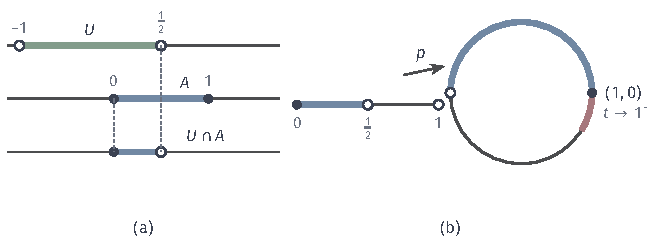
\includegraphics[width=111.774mm]{figures/04-spaces-measures-and-geometry/01-topology-and-metric/tikz/topo-subspace-wrap/figure.pdf}
  \caption{子空间中的相对开集。(a)绿色的$U=(-1,1/2)$在$\mathbb R$中开，与蓝色的$A=[0,1]$相交得到$[0,1/2)$，它在$A$中相对开，在$\mathbb R$中不开。(b)$p$把$[0,1/2)$（蓝色）绕成上半圆弧，弧含$(1,0)$；$(1,0)$下方的点（红色）来自$t$接近$1$的参数，不在弧上，所以弧不相对开。}
  \label{fig:topo-subspace-wrap}
\end{BookInlineFigure}

\subsection{有限乘积}
\label{sec:topo-finite-products}

描述平面上的位置需要两个实坐标，描述一个随时间变化的位置需要“空间中的点”与“时刻”两个分量。这类成对的数据取值于乘积集合$X\times Y$，我们需要在其上规定开集，使“两个分量都在各自的附近”成为乘积中的附近。

\begin{definition}[乘积拓扑]
\label{def:topo-product}
设$X,Y$是拓扑空间。下面的族生成的拓扑称为$X\times Y$上的\term{乘积拓扑}（product topology）：
\begin{equation}
 \mathcal B=\{U\times V:U\text{在}X\text{中开},\ V\text{在}Y\text{中开}\}.
 \label{eq:topo-product-basis}
\end{equation}
有限个空间$X_1\times\cdots\times X_n$的乘积拓扑同样由$U_1\times\cdots\times U_n$生成。
\end{definition}

$\mathcal B$满足定理~\ref{thm:topo-basis-criterion}的条件：$X\times Y$本身属于$\mathcal B$，并且
\[
 (U_1\times V_1)\cap(U_2\times V_2)=(U_1\cap U_2)\times(V_1\cap V_2)
\]
仍属于$\mathcal B$。

乘积拓扑的开集一般不是“开集乘开集”，而是这些开矩形的并，例如$\mathbb R^2$中的开圆盘。取$X=Y=\mathbb R$，这正是例~\ref{ex:topo-intervals-rectangles}中由开矩形生成的通常拓扑。若$X,Y$分别有拓扑基$\mathcal B_X,\mathcal B_Y$，则$\{B\times B':B\in\mathcal B_X,\ B'\in\mathcal B_Y\}$也是乘积拓扑的基。

\paragraph{投影与分量}
坐标投影$\pi_X(x,y)=x$与$\pi_Y(x,y)=y$是连续的：$\pi_X^{-1}(U)=U\times Y$是基本开集。它们也是开映射，因为基本开集$U\times V$（$V\neq\varnothing$）的像是开集$U$。

乘积拓扑是使两个投影都连续的最粗拓扑：若投影连续，$U\times Y$与$X\times V$必须开，它们的交$U\times V$也就必须开，图~\ref{fig:topo-product-neighborhood}(a)画的就是这个交。这一性质给出下面的判据。

\begin{theorem}[映入乘积的映射]
\label{thm:topo-map-into-product}
设$f:Z\to X\times Y$，写作$f(z)=(f_1(z),f_2(z))$，其中$f_1=\pi_X\circ f$，$f_2=\pi_Y\circ f$。则$f$连续，当且仅当$f_1$与$f_2$都连续。
\end{theorem}
\begin{proof}
若$f$连续，$f_1,f_2$是连续映射的复合，因而连续。

反过来，设$f_1,f_2$连续。对基本开集$U\times V$，有
\[
 f^{-1}(U\times V)=f_1^{-1}(U)\cap f_2^{-1}(V),
\]
这是两个开集的交，因而开。任意开集是基本开集之并，其原像是这些原像之并，所以$f$连续。
\end{proof}

由此，$\mathbb R^n$中的映射可以逐坐标判断连续性，上一小节的$p(t)=(\cos2\pi t,\sin2\pi t)$连续，正是因为两个分量都是连续实函数。这个判据只对映入乘积的映射成立。从乘积出发的映射，即使对每个分量单独连续，也未必整体连续：
\[
 f(x_1,x_2)=\frac{x_1x_2}{x_1^2+x_2^2}\quad(\text{原点处补定义为}0)
\]
在固定任一分量时对另一分量连续，沿对角线$x_1=x_2\neq0$却恒为$1/2$，所以在原点不连续。

\paragraph{空间与区间的乘积}
设$X$是拓扑空间，$I=[0,1]$取$\mathbb R$的子空间拓扑。乘积$X\times I$的点$(x,t)$可以理解为“时刻$t$时位于$x$”。一个连续映射$H:X\times I\to Y$同时记录了一族映射$H_t=H(\cdot,t):X\to Y$，$t\in I$。

乘积拓扑保证这族映射随$t$连续变化：如图~\ref{fig:topo-product-neighborhood}(b)，$(x,t)$的邻域含形如$U\times(t-\delta,t+\delta)$的基本开集（在$I$的端点处只取单侧），所以$x$附近、$t$附近的输入都映到$H(x,t)$附近。每个$H_t$连续，是因为它是$H$与连续映射$x\mapsto(x,t)$的复合。

\begin{BookInlineFigure}
  \centering
  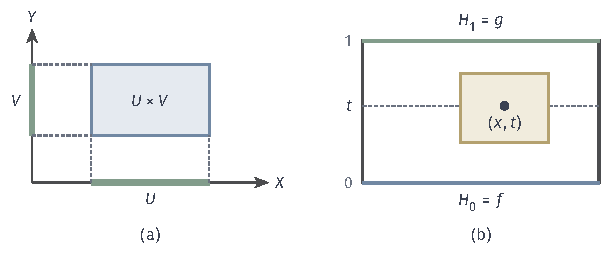
\includegraphics[width=102.404mm]{figures/04-spaces-measures-and-geometry/01-topology-and-metric/tikz/topo-product-neighborhood/figure.pdf}
  \caption{乘积拓扑的基本开集。(a)$U\times V$是投影下$U$与$V$的原像之交。(b)$X\times I$中$H_0=f$在底边，$H_1=g$在顶边，虚线是某一时刻的$H_t$；黄色方块是$(x,t)$的基本开邻域，同时限制空间位置与时刻。}
  \label{fig:topo-product-neighborhood}
\end{BookInlineFigure}

例如，对两个连续映射$f,g:X\to\mathbb R^n$，令
\[
 H(x,t)=(1-t)f(x)+tg(x).
\]
由定理~\ref{thm:topo-map-into-product}，$(x,t)\mapsto(f(x),g(x),t)$连续，$H$的每个坐标是这些分量经实数加法、乘法得到的，加法与乘法作为$\mathbb R^2\to\mathbb R$的映射连续，所以$H$连续。这时$H_0=f$，$H_1=g$，$H$把$f$逐渐变成$g$。

这种从一个映射连续变形到另一个映射的对象称为同伦，它是第~\ref{chap:homology}章的出发点，乘积$X\times I$正是它的定义域。

\subsection{商空间}
\label{sec:topo-quotients}

把一张纸条的两端粘起来，得到一个圈；把正方形的对边分别粘合，得到一个环面。这类构造把原空间中若干点看作同一点，然后问：粘合后的集合上，哪些子集应当算开集？

\paragraph{等价类与投影}
用等价关系$\sim$描述“看作同一点”：$x\sim y$表示$x$与$y$被识别。设$X/{\sim}$为全体等价类$[x]=\{y\in X:y\sim x\}$组成的集合，$q:X\to X/{\sim}$，$q(x)=[x]$，为把每点送到所在类的投影。我们希望$q$连续，而且在这一前提下尽可能多地保留开集。

\begin{definition}[商拓扑]
\label{def:topo-quotient}
设$X$是拓扑空间，$\sim$是$X$上的等价关系。规定$V\subseteq X/{\sim}$为开集，当且仅当$q^{-1}(V)$是$X$的开集。这样得到的拓扑称为\term{商拓扑}（quotient topology），$X/{\sim}$配上商拓扑称为\term{商空间}（quotient space），$q$称为\term{商映射}（quotient map）。
\end{definition}

原像与并、交相容，所以这个族满足拓扑的三条规则。按定义$q$连续，并且商拓扑是使$q$连续的最细拓扑：若$X/{\sim}$上的某个拓扑使$q$连续，它的每个开集$V$都满足$q^{-1}(V)$开，从而属于商拓扑。

子空间、乘积用“最粗”，商空间用“最细”，方向相反的原因在于新拓扑所在的一侧。包含映射与投影的新拓扑在定义域一侧，开集越多映射越容易连续，连续性只给出开集的下限，所以取满足下限的最粗者。商映射的新拓扑在值域一侧，开集越少映射越容易连续，连续性只给出开集的上限，所以取满足上限的最细者。

$q^{-1}(V)$是若干完整等价类之并，所以商空间的开集恰好对应$X$中由完整的类组成的开集。

\begin{example}[区间端点粘合成圆]
\label{ex:topo-interval-gluing-circle}
在$I=[0,1]$上令$0\sim1$，其余每点只与自身等价。等价类为$\{0,1\}$与单点集$\{t\}$（$0<t<1$）。

对内部的点$t$，它在商空间中的邻域就是$I$中$t$附近小区间的像。对粘合点$[0]=\{0,1\}$，集合$V$是它的开邻域，当且仅当$q^{-1}(V)$是含$0$与$1$的开集，因而包含某个$[0,\varepsilon)\cup(1-\varepsilon,1]$。

粘合点的邻域由区间两端的小段拼成，$[0]$两侧都有邻域，这正是例~\ref{ex:topo-interval-to-circle}中$[0,1)$缺少而圆周具有的结构。
\end{example}

取$\varepsilon=0.1$，用$p(t)=(\cos2\pi t,\sin2\pi t)$看，$[0,0.1)$绕出角度$[0^\circ,36^\circ)$，$(0.9,1]$绕出角度$(324^\circ,360^\circ]$。图~\ref{fig:topo-quotient-circle}中，两段在粘合点处接成一段连续的弧，这段弧恰好是圆周上$(1,0)$的开邻域。

\begin{BookInlineFigure}
  \centering
  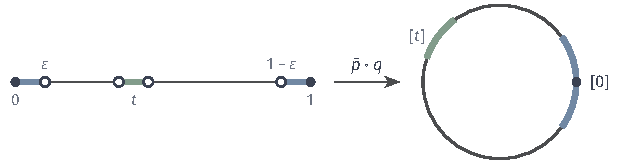
\includegraphics[width=105.11mm]{figures/04-spaces-measures-and-geometry/01-topology-and-metric/tikz/topo-quotient-circle/figure.pdf}
  \caption{区间端点粘合成圆，图中$\varepsilon=0.1$，$t=0.4$。蓝色的两段$[0,\varepsilon)$与$(1-\varepsilon,1]$在粘合后接成粘合点$[0]$的一段开邻域；绿色的小区间对应内部点$[t]$的开邻域。}
  \label{fig:topo-quotient-circle}
\end{BookInlineFigure}

\paragraph{从商空间出发的映射}
商空间上的映射通常是这样得到的：先在$X$上写出一个映射，再检验它在每个等价类上取同一个值。连续性则可以回到$X$上判断。

\begin{theorem}[商空间上的映射]
\label{thm:topo-quotient-maps}
设$q:X\to X/{\sim}$为商映射，$Z$为拓扑空间。
\begin{enumerate}
  \item 映射$g:X/{\sim}\to Z$连续，当且仅当$g\circ q:X\to Z$连续；
  \item 若$f:X\to Z$连续，并且$x\sim y$时$f(x)=f(y)$，则存在唯一的连续映射$\bar f:X/{\sim}\to Z$使$\bar f\circ q=f$。
\end{enumerate}
\end{theorem}
\begin{proof}
对$Z$的开集$W$，有
\[
 q^{-1}\bigl(g^{-1}(W)\bigr)=(g\circ q)^{-1}(W).
\]
按商拓扑的定义，$g^{-1}(W)$开当且仅当左边开，第一条成立。

对第二条，令$\bar f([x])=f(x)$。$f$在每个类上取同一个值，所以这个定义不依赖代表元的选择，并且$\bar f\circ q=f$。$q$是满射，满足这个等式的映射只能是$\bar f$。由$\bar f\circ q=f$连续及第一条，$\bar f$连续。
\end{proof}

把定理用于例~\ref{ex:topo-interval-gluing-circle}：$p:I\to S^1$连续且$p(0)=p(1)$，于是诱导出连续映射$\bar p:I/{\sim}\to S^1$。$p$在$(0,1)$上单射，并且只有$0,1$两点映到$(1,0)$，所以$\bar p$是双射。

到这里得到的只是连续双射。要说明$\bar p^{-1}$也连续，还需要关于紧性和分离性的工具，第~\ref{sec:topo-compact-images}小节完成这一步。另一方面，粘合可能破坏“不同点能用开集分开”这一性质，第~\ref{sec:topo-separation}小节会给出这样的商空间。
